\section{General Overview of Fides}
\label{sec:general-overview-of-fides}
In this section we describe how does Fides work from the high level perspective. We will be referencing chapters and sections further into the thesis that provide more information and describe particular situations and solutions in more detail.

\begin{figure}[ht!]
    \centering
    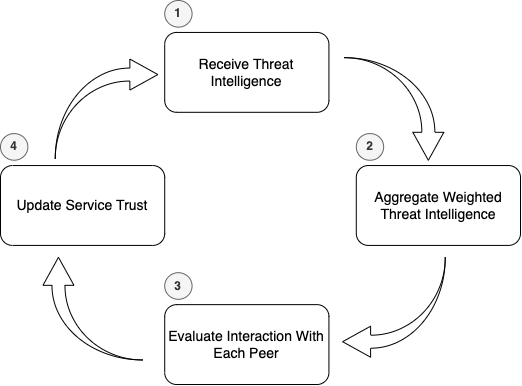
\includegraphics[width=0.75\textwidth]{assets/service_trust_diagram.png}
    \caption{Trust Model Life Cycle}
    \label{fig:trust-model-life-cycle}
\end{figure}

Fides operates in four phases, which are visualized in the figure \ref{fig:trust-model-life-cycle}.
In the first phase, local Fides's instance receives threat intelligence data from the remote peers in the network. 
How Fides receives data from the network is described in the chapter about architecture \ref{ch:architecture}.

In the second phase, Fides aggregates the threat intelligence data utilizing the trust data it has for each remote peer during the aggregation.
In general, data from high trusted peers have a higher impact on the final aggregated threat intelligence than the data from peers with low trust.
How does Fides do that is described in the section  \ref{sec:network-intelligence-aggregation}.
This aggregated threat intelligence is also sent to Slips as an output of the trust model.

The following phase is when Fides evaluates the interactions with each peer.
Fides computes how much it was satisfied with threat intelligence it received from each remote peer.
This satisfaction metric has then a direct influence on the trust relationship between the local and remote peers because it is used in the next step to compute trust data. 
The evaluation process and possible interaction evaluation functions are described in detail in section \ref{sec:interaction-evaluation-strategies}.

In the last step, Fides updates trust data for each peer according to the satisfaction that is computed in step number three.
Computations that allow Fides to do that are described in detail in section \ref{sec:computational-model}.

\todo[inline]{add that awesome diagram from Sebas}